\documentclass{standalone}
\usepackage{tikz}
\usepackage{bm}
\usetikzlibrary{fit,positioning}
\begin{document}
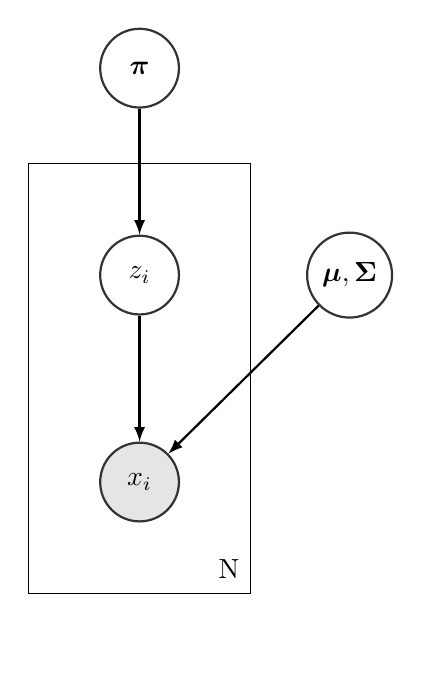
\begin{tikzpicture}
\tikzstyle{main}=[circle, minimum size = 10mm, thick, draw =black!80, node distance = 16mm]
\tikzstyle{connect}=[-latex, thick]
\tikzstyle{box}=[rectangle, draw=black!100]
  \node[main] (pi) [] { $\bm{\pi}$ };
  \node[main] (z) [below=of pi] { $z_i$ };
  \node[main] (theta) [right=of z] { $\bm{\mu}, \bm{\Sigma}$ };
  \node[main, fill = black!10] (f) [below=of z] { $x_{i}$ };
  \path (pi) edge [connect] (z)
        (z) edge [connect] (f)
        (theta) edge [connect] (f);
  %\node[rectangle, inner sep=0mm, fit= (f),label=below right:D, xshift=-1mm, yshift=1mm] {};
  %\node[rectangle, inner sep=4.4mm,draw=black!100, fit= (f)] {};
  \node[rectangle, inner sep=4.6mm, fit= (z) (f),label=below right:N, xshift=-1mm, yshift=-12mm] {};
  \node[rectangle, inner sep=9mm, draw=black!100, fit = (z) (f)] {};
\end{tikzpicture}
\end{document}
